%% This is an example first chapter.  You should put chapter/appendix that you
%% write into a separate file, and add a line \include{yourfilename} to
%% main.tex, where `yourfilename.tex' is the name of the chapter/appendix file.
%% You can process specific files by typing their names in at the 
%% \files=
%% prompt when you run the file main.tex through LaTeX.

\singlespacing{

\chapter{Introduction}

A moonshot goal of digital fabrication is the bottom up programmable assembly of meter scale objects with nanometer scale precision.  With this technology, we could design materials with exotic physical properties and radically transform the way we make almost anything.  We believe this is possible by constructing nanoscale assemblers that work together to precisely control and place raw material feedstock.  Though it sounds like science fiction, biology has demonstrated that this is possible.  Data encoded in DNA can be executed like a computer program to build an immense assortment of molecular-scale machines, which together, coordinate the higher level structure and functions of an organism.
\\

Other parallels between biological assembly and our proposed system are the discretization of a relatively small number of different feedstocks and parallelization of assembly.  The protein machinery of biology is made primarily from the same basis set of 20 amino acids, yet proteins display a wide variety of functions and morphologies to carry out the many tasks of the cell in parallel.  Similarly, the material feedstock of the nano-assemblers consists of a finite set of part types, called "digital materials".  These digital materials are joined together in various patterns to produce diverse, functional structures.  Since construction takes place one nano-brick at a time, many assemblers would need to work in parallel to build structures of any significant size.  If the assemblers are designed in such a way that they can be constructed from their own feedstock, assemblers can build more assemblers and the rate of assembly scales exponentially.
\\

\begin{figure}
  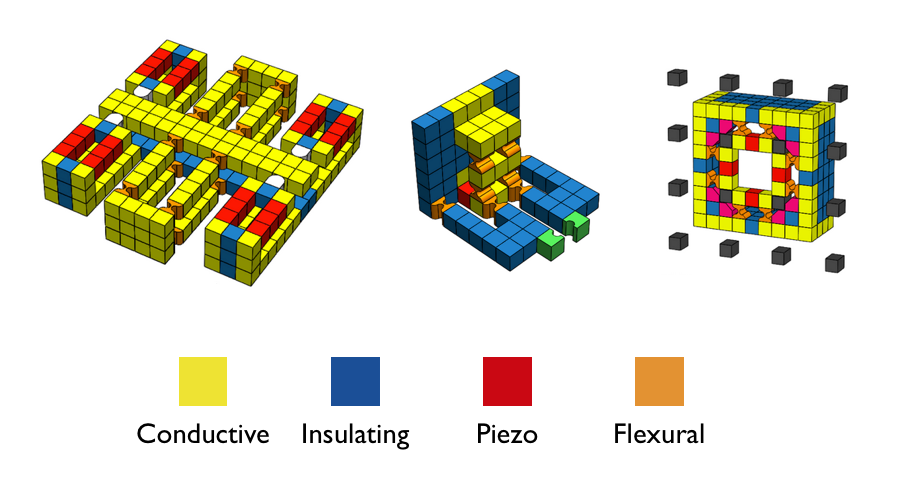
\includegraphics[width=\linewidth]{willMockups.png}
  \caption{Design mock-ups of assembler components made from digital materials by Will Langford.  From left to right: a linear actuator, a part gripping mechanism, a clamping mechanism.  None of these designs has been evaluated in simulation.}
  \label{fig:willMockups}
\end{figure}
The nano-assembly I've described will look very different from the way we make things today, and opposes many of the assumptions baked into traditional Computer Aided Design (CAD),  Computer Aided Manufacturing (CAM), and robotics.  This assembly strategy follows from an existing line of research called "digital assembly", where discrete parts are assembled on a regular, periodic lattice.  Mechanical systems are built with discrete modules of rigid and flexural components, and electronics and controls are distributed spatially across a machine (Fig \ref{fig:willMockups}).  Large structures appear to be "living" in the sense that their surface is teeming with nano-robots, detecting and correcting errors and performing other functions.  The environment is highly structured, allowing locomotion systems to position themselves globally by counting local movements across a lattice.  Machines receive instructions from their environment to coordinate various tasks.
\\

\section{Motivation}

The main contribution of this work is to create a design/simulation environment where anyone can start to explore the rich design space around digital materials in a physically realistic way.  This work will inform future trajectories in CBA research and in the broader field of programmable materials, modular robotics, and digital fabrication.  This work is not intended to result in a manual outlining all the necessary components for self-replication based on current technology, but rather as an sandbox for exploring self-assembling systems based on the foundations of engineering and materials science rather than biology.

\subsection{Nano-Fabrication}

Initial investigations 

\subsubsection{New Materials and Improved Material Performance}

Nano structures allow for physical phenomena that are normally confined to the nanoscale to be accessed at the macroscale.  Gecko paper
nano structures affect the bulk material properties of macro-scale objects - strength, stiffness, friction, porosity, filtering, hydrophobicity, self cleaning, adhesion, conductivity...

\subsubsection{Decreased Cost}

relative cost of biological nano products - wood, down, bomb-sniffing dogs
use of microbes to produce chemicals with high efficiency - insullin etc

cost of nano-fabrication facitily, vibration specs, build size of machines, resolution

\subsubsection{Exponential Growth}

machines make machines

\subsection{Multiphysics for the Masses}

ease of minecraft design + physical reality
